% This file was created by matplotlib v0.1.0.
% Copyright (c) 2010--2014, Nico Schlömer <nico.schloemer@gmail.com>
% All rights reserved.
%
% The lastest updates can be retrieved from
%
% https://github.com/nschloe/matplotlib2tikz
%
% where you can also submit bug reports and leavecomments.
%
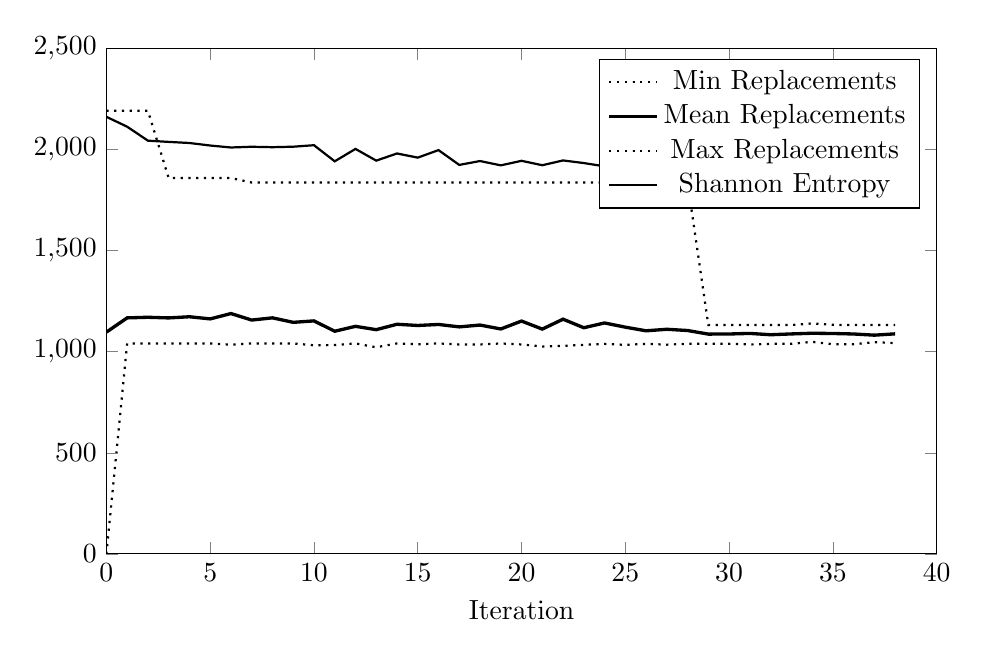
\begin{tikzpicture}[trim left=-1cm]

\definecolor{color1}{rgb}{0.75,0,0.75}
\definecolor{color0}{rgb}{0,0.75,0.75}

\begin{axis}[
width=\textwidth,
height=8cm,
xlabel={Iteration},
xmin=0, xmax=40,
ymin=0, ymax=2500,
axis on top,
legend entries={{Min Replacements},{Mean Replacements},{Max Replacements},{Shannon Entropy}}
]
\addplot [dotted, thick]
coordinates {
(0,0)
(1,1041)
(2,1041)
(3,1041)
(4,1041)
(5,1041)
(6,1035)
(7,1041)
(8,1041)
(9,1041)
(10,1032)
(11,1033)
(12,1041)
(13,1022)
(14,1041)
(15,1037)
(16,1041)
(17,1036)
(18,1036)
(19,1041)
(20,1036)
(21,1026)
(22,1029)
(23,1034)
(24,1039)
(25,1034)
(26,1039)
(27,1035)
(28,1039)
(29,1039)
(30,1039)
(31,1036)
(32,1039)
(33,1039)
(34,1049)
(35,1037)
(36,1037)
(37,1047)
(38,1043)

};
\addplot [very thick]
coordinates {
(0,1097.02)
(1,1167.5)
(2,1170.46)
(3,1167.3)
(4,1173.06)
(5,1162.42)
(6,1188.86)
(7,1156.68)
(8,1167.62)
(9,1145.42)
(10,1152.54)
(11,1101.42)
(12,1125.64)
(13,1109.14)
(14,1135.9)
(15,1129.9)
(16,1134.92)
(17,1122.94)
(18,1131.98)
(19,1112.54)
(20,1151.82)
(21,1111.92)
(22,1161.02)
(23,1118.76)
(24,1142.36)
(25,1121.54)
(26,1103.54)
(27,1111.1)
(28,1104.96)
(29,1087.2)
(30,1087.72)
(31,1090.6)
(32,1084.1)
(33,1088.1)
(34,1091.42)
(35,1090.22)
(36,1087.78)
(37,1081.96)
(38,1088.46)

};
\addplot [dotted, thick]
coordinates {
(0,2192)
(1,2192)
(2,2192)
(3,1859)
(4,1859)
(5,1859)
(6,1859)
(7,1837)
(8,1837)
(9,1837)
(10,1837)
(11,1837)
(12,1837)
(13,1837)
(14,1837)
(15,1837)
(16,1837)
(17,1837)
(18,1837)
(19,1837)
(20,1837)
(21,1837)
(22,1837)
(23,1837)
(24,1837)
(25,1837)
(26,1837)
(27,1837)
(28,1837)
(29,1132)
(30,1132)
(31,1132)
(32,1132)
(33,1132)
(34,1140)
(35,1133)
(36,1132)
(37,1132)
(38,1132)

};
\addplot [thick]
coordinates {
(0,2161.99621997945)
(1,2113.16085166022)
(2,2044.0750730143)
(3,2038.0140648874)
(4,2032.53960838096)
(5,2020.04520219301)
(6,2010.34741350398)
(7,2013.92601030156)
(8,2011.79579941526)
(9,2014.22414629607)
(10,2021.64211590226)
(11,1941.97318640824)
(12,2003.27334175338)
(13,1945.3392499272)
(14,1980.72149513039)
(15,1960.19722982837)
(16,1997.33007483401)
(17,1924.12932437937)
(18,1943.32301881714)
(19,1921.91272972286)
(20,1944.42666980454)
(21,1922.58850126645)
(22,1946.30162048225)
(23,1933.32937733597)
(24,1917.20356309781)
(25,1908.60941099222)
(26,1927.3289273151)
(27,1953.64801029677)
(28,1895.09947644068)
(29,1910.33446002315)
(30,1898.38548773066)
(31,1879.52656299292)
(32,1853.97824096427)
(33,1887.86495554381)
(34,1881.46626968771)
(35,1873.32515826854)
(36,1837.06860937504)
(37,1878.17969872628)
(38,1872.78187219633)

};
\path [draw=black, fill opacity=0] (axis cs:13,2500)--(axis cs:13,2500);

\path [draw=black, fill opacity=0] (axis cs:40,13)--(axis cs:40,13);

\path [draw=black, fill opacity=0] (axis cs:13,0)--(axis cs:13,0);

\path [draw=black, fill opacity=0] (axis cs:0,13)--(axis cs:0,13);

\end{axis}

\end{tikzpicture}
